	\subsection{UC 8 - Gestione alert ente}
		
		\begin{figure}[H]
			\centering
			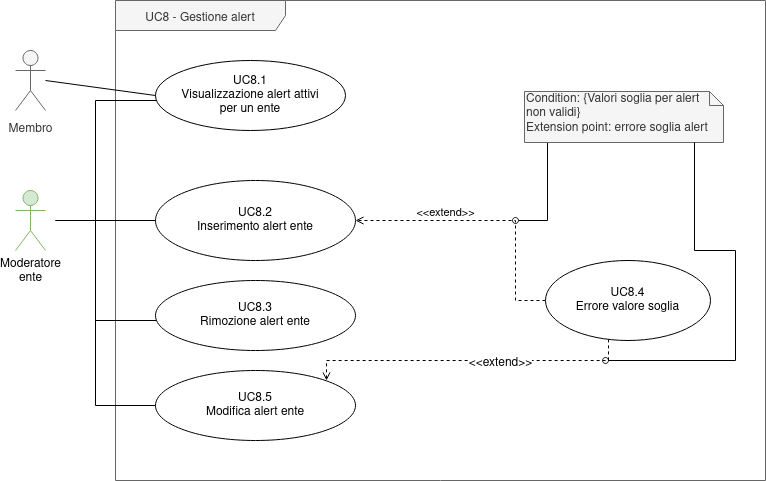
\includegraphics[scale=0.60]{res/images/uc8}
			\caption{Diagramma che descrive gli alert da abilitare per un singolo ente.}
		\end{figure}

		\begin{itemize}
			\item \textbf{attori primari:} Membro, Moderatore ente;
			\item \textbf{descrizione:} l'utente gestisce gli \glock{alert} del proprio ente, impostandone le soglie oltre il quale scatenare le notifiche per gli utenti;
			\item \textbf{precondizione:} l'utente è autenticato e naviga all'interno della gestione \glock{alert};
			\item \textbf{postcondizione:} l'utente ha visualizzato o gestito gli \glock{alert} del proprio ente;
			\item \textbf{scenario principale:}
			\begin{enumerate}
				\item{l'utente naviga all'interno della gestione \glock{alert} del proprio ente;}
				\item{l'utente ha visualizzato o gestito gli \glock{alert} del proprio ente.}
			\end{enumerate}	
		\end{itemize}
			
			\subsubsection{UC 8.1 - Visualizzazione alert ente}
			\begin{itemize}
				\item \textbf{attori primari:} Membro, Moderatore ente;
				\item \textbf{descrizione:} l'utente può visualizzare il nome del sensore e la soglia degli \glock{alert} appartenenti al proprio ente;
				\item \textbf{precondizione:} l'utente naviga all'interno della gestione \glock{alert};
				\item \textbf{postcondizione:} l'utente ha visualizzato la lista degli \glock{alert} del proprio ente;
				\item \textbf{scenario principale:}
				\begin{enumerate}
					\item{l'utente visualizza la lista degli \glock{alert} del proprio ente.}
				\end{enumerate}	
			\end{itemize}
			
			\subsubsection{UC 8.2 - Inserimento alert ente}
			\begin{itemize}
				\item \textbf{attori primari:} Moderatore ente;
				\item \textbf{descrizione:} l'utente può inserire un nuovo \glock{alert} per il proprio ente;
				\item \textbf{precondizione:} l'utente naviga all'interno della gestione \glock{alert};
				\item \textbf{postcondizione:} l'utente ha inserito un nuovo \glock{alert} per gli utenti appartenenti al proprio ente;
				\item \textbf{scenario principale:}
				\begin{enumerate}
					\item{l'utente compila i campi con i dati dell'\glock{alert} da inserire;}
					\item l'utente seleziona un sensore tra quelli disponibile su cui eseguire il controllo (UC 8.2.1);
					\item l'utente inserisce una soglia da controllare per il sensore (UC 8.2.2);
					\item{l'utente ha inserito un nuovo \glock{alert} per gli utenti appartenenti al proprio ente;}
				\end{enumerate}
				\item \textbf{estensioni:}
				\begin{itemize}
					\item l'utente inserisce dei valori soglia non validi (UC 8.4).
				\end{itemize}		
			\end{itemize}
			
				\paragraph{UC 8.2.1 - Selezione sensore per nuovo alert}
				\begin{itemize}
					\item \textbf{attori primari:} Moderatore ente;
					\item \textbf{descrizione:} l'utente compila un campo per l'inserimento di un nuovo \glock{alert} e in particolare seleziona un sensore su cui eseguire il controllo;
					\item \textbf{precondizione:} l'utente sta inserendo i dati per un nuovo \glock{alert};
					\item \textbf{postcondizione:} l'utente ha compilato il campo richiesto;
					\item \textbf{scenario principale:}
					\begin{enumerate}
						\item{l'utente seleziona il sensore disponibile da verificare tra un elenco di quelli disponibili.}
					\end{enumerate}	
				\end{itemize}

				\paragraph{UC 8.2.2 - Inserimento soglia per nuovo alert}
				\begin{itemize}
					\item \textbf{attori primari:} Moderatore ente;
					\item \textbf{descrizione:} l'utente compila un campo per l'inserimento di un nuovo \glock{alert} e in particolare seleziona la soglia da controllare;
					\item \textbf{precondizione:} l'utente sta inserendo i dati per un nuovo \glock{alert};
					\item \textbf{postcondizione:} l'utente ha compilato il campo richiesto;
					\item \textbf{scenario principale:}
					\begin{enumerate}
						\item{l'utente inserisce la soglia del sensore da verificare.}
					\end{enumerate}	
				\end{itemize}

			\subsubsection{UC 8.3 - Rimozione alert ente}
			\begin{itemize}
				\item \textbf{attori primari:} Moderatore ente;
				\item \textbf{descrizione:} l'utente può rimuovere un \glock{alert} selezionandolo dalla lista degli \glock{alert} attivi del proprio ente;
				\item \textbf{precondizione:} l'utente naviga all'interno della gestione \glock{alert} e ha disponibile almeno un alert;
				\item \textbf{postcondizione:} l'utente ha rimosso l'\glock{alert} selezionato del proprio ente dal sistema;
				\item \textbf{scenario principale:}
				\begin{enumerate}
					\item{l'utente seleziona un \glock{alert} dalla lista degli \glock{alert} del proprio ente e lo rimuove;}
					\item{l'utente non visualizza più l'\glock{alert} selezionato.}
				\end{enumerate}	
			\end{itemize}

			\subsubsection{UC 8.4 - Errore valore soglia}
			\begin{itemize}
				\item \textbf{attori primari:} Moderatore ente;
				\item \textbf{descrizione:} dopo aver premuto il bottone per confermare i campi inseriti, viene visualizzato il messaggio di errore che segnala un valore soglia non valido;
				\item \textbf{precondizione:} l'utente ha inserito i campi richiesti e il sistema sta elaborando la richiesta;
				\item \textbf{postcondizione:} visualizzazione messaggio di errore specifico;
				\item \textbf{scenario principale:}
				\begin{enumerate}
					\item{il sistema elabora la richiesta;}
					\item{viene visualizzato il messaggio di errore che spiega che il valore soglia inserito per un \glock{alert} non è valido.}
				\end{enumerate}
			\end{itemize}
			
			\subsubsection{UC 8.5 - Modifica alert ente}
			\begin{itemize}
				\item \textbf{attori primari:} Moderatore ente;
				\item \textbf{descrizione:} l'utente può modificare \glock{alert} esistente per il proprio ente;
				\item \textbf{precondizione:} l'utente naviga all'interno della gestione \glock{alert};
				\item \textbf{postcondizione:} l'utente ha inserito un nuovo \glock{alert} per gli utenti appartenenti al proprio ente;
				\item \textbf{scenario principale:}
				\begin{enumerate}
					\item{l'utente compila i campi con i dati dell'\glock{alert} da inserire;}
					\item l'utente modifica la soglia da controllare per il sensore (UC 8.5.1);
					\item{l'utente ha inserito un nuovo \glock{alert} per gli utenti appartenenti al proprio ente;}
				\end{enumerate}
				\item \textbf{estensioni:}
				\begin{itemize}
					\item l'utente inserisce dei valori soglia non validi (UC 8.4).
				\end{itemize}		
			\end{itemize}

				\paragraph{UC 8.5.1 - Modifica soglia per alert}
				\begin{itemize}
					\item \textbf{attori primari:} Moderatore ente;
					\item \textbf{descrizione:} l'utente compila un campo per la modifica di un \glock{alert} e in particolare inserisce la soglia da controllare;
					\item \textbf{precondizione:} l'utente sta inserendo i dati per modificare un \glock{alert};
					\item \textbf{postcondizione:} l'utente ha compilato il campo richiesto;
					\item \textbf{scenario principale:}
					\begin{enumerate}
						\item{l'utente inserisce la soglia del sensore da verificare.}
					\end{enumerate}	
				\end{itemize}